% Options for packages loaded elsewhere
% Options for packages loaded elsewhere
\PassOptionsToPackage{unicode}{hyperref}
\PassOptionsToPackage{hyphens}{url}
\PassOptionsToPackage{dvipsnames,svgnames,x11names}{xcolor}
%
\documentclass[
  letterpaper,
  DIV=11,
  numbers=noendperiod]{scrartcl}
\usepackage{xcolor}
\usepackage{amsmath,amssymb}
\setcounter{secnumdepth}{-\maxdimen} % remove section numbering
\usepackage{iftex}
\ifPDFTeX
  \usepackage[T1]{fontenc}
  \usepackage[utf8]{inputenc}
  \usepackage{textcomp} % provide euro and other symbols
\else % if luatex or xetex
  \usepackage{unicode-math} % this also loads fontspec
  \defaultfontfeatures{Scale=MatchLowercase}
  \defaultfontfeatures[\rmfamily]{Ligatures=TeX,Scale=1}
\fi
\usepackage{lmodern}
\ifPDFTeX\else
  % xetex/luatex font selection
\fi
% Use upquote if available, for straight quotes in verbatim environments
\IfFileExists{upquote.sty}{\usepackage{upquote}}{}
\IfFileExists{microtype.sty}{% use microtype if available
  \usepackage[]{microtype}
  \UseMicrotypeSet[protrusion]{basicmath} % disable protrusion for tt fonts
}{}
\makeatletter
\@ifundefined{KOMAClassName}{% if non-KOMA class
  \IfFileExists{parskip.sty}{%
    \usepackage{parskip}
  }{% else
    \setlength{\parindent}{0pt}
    \setlength{\parskip}{6pt plus 2pt minus 1pt}}
}{% if KOMA class
  \KOMAoptions{parskip=half}}
\makeatother
% Make \paragraph and \subparagraph free-standing
\makeatletter
\ifx\paragraph\undefined\else
  \let\oldparagraph\paragraph
  \renewcommand{\paragraph}{
    \@ifstar
      \xxxParagraphStar
      \xxxParagraphNoStar
  }
  \newcommand{\xxxParagraphStar}[1]{\oldparagraph*{#1}\mbox{}}
  \newcommand{\xxxParagraphNoStar}[1]{\oldparagraph{#1}\mbox{}}
\fi
\ifx\subparagraph\undefined\else
  \let\oldsubparagraph\subparagraph
  \renewcommand{\subparagraph}{
    \@ifstar
      \xxxSubParagraphStar
      \xxxSubParagraphNoStar
  }
  \newcommand{\xxxSubParagraphStar}[1]{\oldsubparagraph*{#1}\mbox{}}
  \newcommand{\xxxSubParagraphNoStar}[1]{\oldsubparagraph{#1}\mbox{}}
\fi
\makeatother

\usepackage{color}
\usepackage{fancyvrb}
\newcommand{\VerbBar}{|}
\newcommand{\VERB}{\Verb[commandchars=\\\{\}]}
\DefineVerbatimEnvironment{Highlighting}{Verbatim}{commandchars=\\\{\}}
% Add ',fontsize=\small' for more characters per line
\usepackage{framed}
\definecolor{shadecolor}{RGB}{241,243,245}
\newenvironment{Shaded}{\begin{snugshade}}{\end{snugshade}}
\newcommand{\AlertTok}[1]{\textcolor[rgb]{0.68,0.00,0.00}{#1}}
\newcommand{\AnnotationTok}[1]{\textcolor[rgb]{0.37,0.37,0.37}{#1}}
\newcommand{\AttributeTok}[1]{\textcolor[rgb]{0.40,0.45,0.13}{#1}}
\newcommand{\BaseNTok}[1]{\textcolor[rgb]{0.68,0.00,0.00}{#1}}
\newcommand{\BuiltInTok}[1]{\textcolor[rgb]{0.00,0.23,0.31}{#1}}
\newcommand{\CharTok}[1]{\textcolor[rgb]{0.13,0.47,0.30}{#1}}
\newcommand{\CommentTok}[1]{\textcolor[rgb]{0.37,0.37,0.37}{#1}}
\newcommand{\CommentVarTok}[1]{\textcolor[rgb]{0.37,0.37,0.37}{\textit{#1}}}
\newcommand{\ConstantTok}[1]{\textcolor[rgb]{0.56,0.35,0.01}{#1}}
\newcommand{\ControlFlowTok}[1]{\textcolor[rgb]{0.00,0.23,0.31}{\textbf{#1}}}
\newcommand{\DataTypeTok}[1]{\textcolor[rgb]{0.68,0.00,0.00}{#1}}
\newcommand{\DecValTok}[1]{\textcolor[rgb]{0.68,0.00,0.00}{#1}}
\newcommand{\DocumentationTok}[1]{\textcolor[rgb]{0.37,0.37,0.37}{\textit{#1}}}
\newcommand{\ErrorTok}[1]{\textcolor[rgb]{0.68,0.00,0.00}{#1}}
\newcommand{\ExtensionTok}[1]{\textcolor[rgb]{0.00,0.23,0.31}{#1}}
\newcommand{\FloatTok}[1]{\textcolor[rgb]{0.68,0.00,0.00}{#1}}
\newcommand{\FunctionTok}[1]{\textcolor[rgb]{0.28,0.35,0.67}{#1}}
\newcommand{\ImportTok}[1]{\textcolor[rgb]{0.00,0.46,0.62}{#1}}
\newcommand{\InformationTok}[1]{\textcolor[rgb]{0.37,0.37,0.37}{#1}}
\newcommand{\KeywordTok}[1]{\textcolor[rgb]{0.00,0.23,0.31}{\textbf{#1}}}
\newcommand{\NormalTok}[1]{\textcolor[rgb]{0.00,0.23,0.31}{#1}}
\newcommand{\OperatorTok}[1]{\textcolor[rgb]{0.37,0.37,0.37}{#1}}
\newcommand{\OtherTok}[1]{\textcolor[rgb]{0.00,0.23,0.31}{#1}}
\newcommand{\PreprocessorTok}[1]{\textcolor[rgb]{0.68,0.00,0.00}{#1}}
\newcommand{\RegionMarkerTok}[1]{\textcolor[rgb]{0.00,0.23,0.31}{#1}}
\newcommand{\SpecialCharTok}[1]{\textcolor[rgb]{0.37,0.37,0.37}{#1}}
\newcommand{\SpecialStringTok}[1]{\textcolor[rgb]{0.13,0.47,0.30}{#1}}
\newcommand{\StringTok}[1]{\textcolor[rgb]{0.13,0.47,0.30}{#1}}
\newcommand{\VariableTok}[1]{\textcolor[rgb]{0.07,0.07,0.07}{#1}}
\newcommand{\VerbatimStringTok}[1]{\textcolor[rgb]{0.13,0.47,0.30}{#1}}
\newcommand{\WarningTok}[1]{\textcolor[rgb]{0.37,0.37,0.37}{\textit{#1}}}

\usepackage{longtable,booktabs,array}
\newcounter{none} % for unnumbered tables
\usepackage{calc} % for calculating minipage widths
% Correct order of tables after \paragraph or \subparagraph
\usepackage{etoolbox}
\makeatletter
\patchcmd\longtable{\par}{\if@noskipsec\mbox{}\fi\par}{}{}
\makeatother
% Allow footnotes in longtable head/foot
\IfFileExists{footnotehyper.sty}{\usepackage{footnotehyper}}{\usepackage{footnote}}
\makesavenoteenv{longtable}
\usepackage{graphicx}
\makeatletter
\newsavebox\pandoc@box
\newcommand*\pandocbounded[1]{% scales image to fit in text height/width
  \sbox\pandoc@box{#1}%
  \Gscale@div\@tempa{\textheight}{\dimexpr\ht\pandoc@box+\dp\pandoc@box\relax}%
  \Gscale@div\@tempb{\linewidth}{\wd\pandoc@box}%
  \ifdim\@tempb\p@<\@tempa\p@\let\@tempa\@tempb\fi% select the smaller of both
  \ifdim\@tempa\p@<\p@\scalebox{\@tempa}{\usebox\pandoc@box}%
  \else\usebox{\pandoc@box}%
  \fi%
}
% Set default figure placement to htbp
\def\fps@figure{htbp}
\makeatother





\setlength{\emergencystretch}{3em} % prevent overfull lines

\providecommand{\tightlist}{%
  \setlength{\itemsep}{0pt}\setlength{\parskip}{0pt}}



 


\usepackage{fvextra}
\DefineVerbatimEnvironment{Highlighting}{Verbatim}{breaklines,commandchars=\\\{\}}
\DefineVerbatimEnvironment{OutputCode}{Verbatim}{breaklines,commandchars=\\\{\}}
\KOMAoption{captions}{tableheading}
\makeatletter
\@ifpackageloaded{caption}{}{\usepackage{caption}}
\AtBeginDocument{%
\ifdefined\contentsname
  \renewcommand*\contentsname{Table of contents}
\else
  \newcommand\contentsname{Table of contents}
\fi
\ifdefined\listfigurename
  \renewcommand*\listfigurename{List of Figures}
\else
  \newcommand\listfigurename{List of Figures}
\fi
\ifdefined\listtablename
  \renewcommand*\listtablename{List of Tables}
\else
  \newcommand\listtablename{List of Tables}
\fi
\ifdefined\figurename
  \renewcommand*\figurename{Figure}
\else
  \newcommand\figurename{Figure}
\fi
\ifdefined\tablename
  \renewcommand*\tablename{Table}
\else
  \newcommand\tablename{Table}
\fi
}
\@ifpackageloaded{float}{}{\usepackage{float}}
\floatstyle{ruled}
\@ifundefined{c@chapter}{\newfloat{codelisting}{h}{lop}}{\newfloat{codelisting}{h}{lop}[chapter]}
\floatname{codelisting}{Listing}
\newcommand*\listoflistings{\listof{codelisting}{List of Listings}}
\makeatother
\makeatletter
\makeatother
\makeatletter
\@ifpackageloaded{caption}{}{\usepackage{caption}}
\@ifpackageloaded{subcaption}{}{\usepackage{subcaption}}
\makeatother
\usepackage{bookmark}
\IfFileExists{xurl.sty}{\usepackage{xurl}}{} % add URL line breaks if available
\urlstyle{same}
\hypersetup{
  pdftitle={Timeline Check-in},
  pdfauthor={Linda Herrera, Natalie Chen, June McNally},
  colorlinks=true,
  linkcolor={blue},
  filecolor={Maroon},
  citecolor={Blue},
  urlcolor={Blue},
  pdfcreator={LaTeX via pandoc}}


\title{Timeline Check-in}
\author{Linda Herrera, Natalie Chen, June McNally}
\date{}
\begin{document}
\maketitle


\subsection{Set up}\label{set-up}

\subsubsection{Packages}\label{packages}

\begin{Shaded}
\begin{Highlighting}[]
\CommentTok{\# general use and cleaning}
\FunctionTok{library}\NormalTok{(tidyverse)}
\FunctionTok{library}\NormalTok{(here)}
\FunctionTok{library}\NormalTok{(janitor)}
\FunctionTok{library}\NormalTok{(snakecase)}

\CommentTok{\# wrapping axis labels}
\FunctionTok{library}\NormalTok{(scales)}

\CommentTok{\# reading in .xlsx files}
\FunctionTok{library}\NormalTok{(readxl)}

\CommentTok{\# arranging plots}
\FunctionTok{library}\NormalTok{(patchwork)}
\FunctionTok{library}\NormalTok{(ggridges)}
\end{Highlighting}
\end{Shaded}

\subsubsection{Data}\label{data}

\begin{Shaded}
\begin{Highlighting}[]
\CommentTok{\# taxonomic information}
\NormalTok{taxon\_list }\OtherTok{\textless{}{-}} \FunctionTok{read\_csv}\NormalTok{(}\FunctionTok{here}\NormalTok{(}\StringTok{"data"}\NormalTok{, }\StringTok{"taxon\_list.csv"}\NormalTok{)) }

\CommentTok{\# aquatic invertebrates}
\NormalTok{aq\_ins }\OtherTok{\textless{}{-}} \FunctionTok{read\_xlsx}\NormalTok{(}\FunctionTok{here}\NormalTok{(}\StringTok{"data"}\NormalTok{, }\StringTok{"Aquatic Sampling Data{-}2026{-}03{-}10.xlsx"}\NormalTok{),}
                    \AttributeTok{sheet =} \StringTok{"Aquatic Insects"}\NormalTok{) }

\CommentTok{\# site information}
\NormalTok{sites }\OtherTok{\textless{}{-}} \FunctionTok{read\_xlsx}\NormalTok{(}\FunctionTok{here}\NormalTok{(}\StringTok{"data"}\NormalTok{, }\StringTok{"Aquatic Sampling Data{-}2026{-}03{-}10.xlsx"}\NormalTok{),}
                   \AttributeTok{sheet =} \StringTok{"sites"}\NormalTok{)}

\CommentTok{\# water quality information}
\NormalTok{water\_quality }\OtherTok{\textless{}{-}} \FunctionTok{read\_xlsx}\NormalTok{(}\FunctionTok{here}\NormalTok{(}\StringTok{"data"}\NormalTok{, }\StringTok{"Aquatic Sampling Data{-}2026{-}03{-}10.xlsx"}\NormalTok{),}
                           \AttributeTok{sheet =} \StringTok{"Water Quality"}\NormalTok{,}
                           \AttributeTok{na =} \FunctionTok{c}\NormalTok{(}\StringTok{""}\NormalTok{, }\StringTok{"n/a"}\NormalTok{, }\StringTok{"N/A"}\NormalTok{, }\StringTok{"over"}\NormalTok{, }\StringTok{"173+"}\NormalTok{)) }
\end{Highlighting}
\end{Shaded}

\subsection{Cleaning and Wrangling}\label{cleaning-and-wrangling}

\subsubsection{Cleaning}\label{cleaning}

\paragraph{\texorpdfstring{\texttt{sites}
object}{sites object}}\label{sites-object}

\begin{Shaded}
\begin{Highlighting}[]
\CommentTok{\# creating new object from sites}
\NormalTok{ncos\_sites }\OtherTok{\textless{}{-}}\NormalTok{ sites }\SpecialCharTok{|\textgreater{}} 
  \CommentTok{\# filter to only include NCOS sites sampled four times a year}
  \FunctionTok{filter}\NormalTok{(sector }\SpecialCharTok{==} \StringTok{"NCOS"} \SpecialCharTok{\&}\NormalTok{ sampling\_frequency }\SpecialCharTok{==} \StringTok{"Quarterly"}\NormalTok{)}
\end{Highlighting}
\end{Shaded}

\paragraph{\texorpdfstring{\texttt{taxon\_list}
object}{taxon\_list object}}\label{taxon_list-object}

\begin{Shaded}
\begin{Highlighting}[]
\CommentTok{\# creating new clean object from taxon\_list}
\NormalTok{taxon\_list\_clean }\OtherTok{\textless{}{-}}\NormalTok{ taxon\_list }\SpecialCharTok{|\textgreater{}} 
  \CommentTok{\# converting taxon name to snake case (no spaces or capital letters,}
  \CommentTok{\# only underscores)}
  \FunctionTok{mutate}\NormalTok{(}\AttributeTok{verbatim\_name =} \FunctionTok{to\_any\_case}\NormalTok{(verbatim\_name, }\AttributeTok{case =} \StringTok{"snake"}\NormalTok{)) }\SpecialCharTok{|\textgreater{}} 
  \FunctionTok{select}\NormalTok{(verbatim\_name, scientificName)}
\end{Highlighting}
\end{Shaded}

\paragraph{\texorpdfstring{\texttt{water\_quality}
object}{water\_quality object}}\label{water_quality-object}

\begin{Shaded}
\begin{Highlighting}[]
\NormalTok{water\_quality\_clean }\OtherTok{\textless{}{-}}\NormalTok{ water\_quality }\SpecialCharTok{|\textgreater{}} 
  \FunctionTok{clean\_names}\NormalTok{() }\SpecialCharTok{|\textgreater{}} 
  \FunctionTok{semi\_join}\NormalTok{(ncos\_sites, }\AttributeTok{by =} \StringTok{"site"}\NormalTok{) }\SpecialCharTok{|\textgreater{}} 
  \FunctionTok{unite}\NormalTok{(}\StringTok{"date\_site"}\NormalTok{, date, site, }\AttributeTok{remove =} \ConstantTok{TRUE}\NormalTok{) }\SpecialCharTok{|\textgreater{}} 
  \FunctionTok{group\_by}\NormalTok{(date\_site) }\SpecialCharTok{|\textgreater{}} 
  \FunctionTok{summarize}\NormalTok{(}\AttributeTok{med\_ph    =} \FunctionTok{median}\NormalTok{(p\_h, }\AttributeTok{na.rm =} \ConstantTok{TRUE}\NormalTok{),}
            \AttributeTok{med\_sal   =} \FunctionTok{median}\NormalTok{(salinity\_ppt, }\AttributeTok{na.rm =} \ConstantTok{TRUE}\NormalTok{),}
            \AttributeTok{med\_do    =} \FunctionTok{median}\NormalTok{(dissolved\_oxygen\_mg\_l, }\AttributeTok{na.rm =} \ConstantTok{TRUE}\NormalTok{),}
            \AttributeTok{med\_temp  =} \FunctionTok{median}\NormalTok{(temperature\_c, }\AttributeTok{na.rm =} \ConstantTok{TRUE}\NormalTok{)) }\SpecialCharTok{|\textgreater{}}   \CommentTok{\# \textless{}{-}{-} ADD THIS}
  \FunctionTok{ungroup}\NormalTok{() }\SpecialCharTok{|\textgreater{}} 
  \FunctionTok{filter}\NormalTok{(date\_site }\SpecialCharTok{!=} \StringTok{"2022{-}08{-}12\_NVBR"}\NormalTok{)}
\end{Highlighting}
\end{Shaded}

\paragraph{\texorpdfstring{\texttt{aq\_ins}
object}{aq\_ins object}}\label{aq_ins-object}

\begin{Shaded}
\begin{Highlighting}[]
\CommentTok{\# creating new clean object from aquatic inverts}
\NormalTok{aq\_ins\_clean }\OtherTok{\textless{}{-}}\NormalTok{ aq\_ins }\SpecialCharTok{|\textgreater{}} 
  \CommentTok{\# clean column names}
  \FunctionTok{clean\_names}\NormalTok{() }\SpecialCharTok{|\textgreater{}} 
  \CommentTok{\# filtering join: only include sites occurring in ncos\_sites}
  \FunctionTok{semi\_join}\NormalTok{(ncos\_sites, }\AttributeTok{by =} \FunctionTok{c}\NormalTok{(}\StringTok{"site"}\NormalTok{)) }\SpecialCharTok{|\textgreater{}} 
  \CommentTok{\# renaming columns}
  \FunctionTok{rename}\NormalTok{(}\AttributeTok{date =}\NormalTok{ date\_on\_vial) }\SpecialCharTok{|\textgreater{}} 
  \CommentTok{\# select columns of interest}
  \FunctionTok{select}\NormalTok{(date, sample\_type, site,}
\NormalTok{         ostracod,}
\NormalTok{         copepod,}
\NormalTok{         cladocera) }\SpecialCharTok{|\textgreater{}} 
  \CommentTok{\# filter to only include "filtered beaker" samples}
  \FunctionTok{filter}\NormalTok{(sample\_type }\SpecialCharTok{\%in\%} \FunctionTok{c}\NormalTok{(}\StringTok{"FB 250"}\NormalTok{, }\StringTok{"FB250"}\NormalTok{)) }\SpecialCharTok{|\textgreater{}} 
  \CommentTok{\# convert the data frame to long format}
  \FunctionTok{pivot\_longer}\NormalTok{(}\AttributeTok{cols =}\NormalTok{ ostracod}\SpecialCharTok{:}\NormalTok{cladocera,}
               \AttributeTok{names\_to =} \StringTok{"taxon"}\NormalTok{,}
               \AttributeTok{values\_to =} \StringTok{"abundance"}\NormalTok{) }\SpecialCharTok{|\textgreater{}} 
  \CommentTok{\# group by date, site, taxon}
  \FunctionTok{group\_by}\NormalTok{(date, site, taxon) }\SpecialCharTok{|\textgreater{}} 
  \CommentTok{\# calculate average abundance per liter (sum abundance divided by 7.5 liters)}
  \FunctionTok{summarize}\NormalTok{(}\AttributeTok{ave\_lit =} \FunctionTok{sum}\NormalTok{(abundance, }\AttributeTok{na.rm =} \ConstantTok{TRUE}\NormalTok{)}\SpecialCharTok{/}\FloatTok{7.5}\NormalTok{) }\SpecialCharTok{|\textgreater{}} 
  \CommentTok{\# ungroup data frame}
  \FunctionTok{ungroup}\NormalTok{() }\SpecialCharTok{|\textgreater{}} 
  \CommentTok{\# create a new column called \textasciigrave{}date\_site\textasciigrave{} to join with water quality}
  \FunctionTok{unite}\NormalTok{(}\StringTok{"date\_site"}\NormalTok{, date, site, }\AttributeTok{remove =} \ConstantTok{FALSE}\NormalTok{) }\SpecialCharTok{|\textgreater{}} 
  \CommentTok{\# join with water quality}
  \FunctionTok{left\_join}\NormalTok{(water\_quality\_clean, }\AttributeTok{by =} \FunctionTok{c}\NormalTok{(}\StringTok{"date\_site"}\NormalTok{)) }\SpecialCharTok{|\textgreater{}} 
  \CommentTok{\# join with taxon list}
  \FunctionTok{left\_join}\NormalTok{(taxon\_list\_clean, }\AttributeTok{by =} \FunctionTok{c}\NormalTok{(}\StringTok{"taxon"} \OtherTok{=} \StringTok{"verbatim\_name"}\NormalTok{)) }\SpecialCharTok{|\textgreater{}} 
  \CommentTok{\# add full names of sites}
  \FunctionTok{mutate}\NormalTok{(}\AttributeTok{site\_full =} \FunctionTok{case\_when}\NormalTok{(}
\NormalTok{    site }\SpecialCharTok{==} \StringTok{"NVBR"} \SpecialCharTok{\textasciitilde{}} \StringTok{"North of Venoco Bridge"}\NormalTok{,}
\NormalTok{    site }\SpecialCharTok{==} \StringTok{"NEC"} \SpecialCharTok{\textasciitilde{}} \StringTok{"South of Venoco Bridge"}\NormalTok{,}
\NormalTok{    site }\SpecialCharTok{==} \StringTok{"NMC"} \SpecialCharTok{\textasciitilde{}} \StringTok{"Main Channel"}\NormalTok{,}
\NormalTok{    site }\SpecialCharTok{==} \StringTok{"NPB"} \SpecialCharTok{\textasciitilde{}} \StringTok{"South of Phelps Bridge"}\NormalTok{,}
\NormalTok{    site }\SpecialCharTok{==} \StringTok{"NPB1"} \SpecialCharTok{\textasciitilde{}} \StringTok{"North of Phelps Bridge"}\NormalTok{,}
\NormalTok{    site }\SpecialCharTok{==} \StringTok{"NPB2"} \SpecialCharTok{\textasciitilde{}} \StringTok{"Phelps Road"}\NormalTok{,}
\NormalTok{    site }\SpecialCharTok{==} \StringTok{"NWP"} \SpecialCharTok{\textasciitilde{}}  \StringTok{"West Pond"}\NormalTok{,}
\NormalTok{    site }\SpecialCharTok{==} \StringTok{"NDC"} \SpecialCharTok{\textasciitilde{}} \StringTok{"Devereux Creek"}
\NormalTok{  )) }\SpecialCharTok{|\textgreater{}} 
  \CommentTok{\# setting factor levels for site}
  \FunctionTok{mutate}\NormalTok{(}\AttributeTok{site\_full =} \FunctionTok{fct\_reorder}\NormalTok{(site\_full, med\_sal, }\AttributeTok{.fun =} \StringTok{"median"}\NormalTok{, }\AttributeTok{.na\_rm =} \ConstantTok{TRUE}\NormalTok{),}
         \AttributeTok{site\_full =} \FunctionTok{fct\_rev}\NormalTok{(site\_full)) }\SpecialCharTok{|\textgreater{}} 
  
  \CommentTok{\# ADD: log+1 transform of average abundance per liter}
  \FunctionTok{mutate}\NormalTok{(}\AttributeTok{log\_ave\_lit =} \FunctionTok{log}\NormalTok{(ave\_lit }\SpecialCharTok{+} \DecValTok{1}\NormalTok{)) }\SpecialCharTok{|\textgreater{}}                        \CommentTok{\# \textless{}{-}{-} Fig 1, 2, 3, 4}
  
  \CommentTok{\# ADD: season derived from date}
  \FunctionTok{mutate}\NormalTok{(}\AttributeTok{season =} \FunctionTok{case\_when}\NormalTok{(}
    \FunctionTok{month}\NormalTok{(date) }\SpecialCharTok{\%in\%} \FunctionTok{c}\NormalTok{(}\DecValTok{3}\NormalTok{, }\DecValTok{4}\NormalTok{, }\DecValTok{5}\NormalTok{)  }\SpecialCharTok{\textasciitilde{}} \StringTok{"Spring"}\NormalTok{,}
    \FunctionTok{month}\NormalTok{(date) }\SpecialCharTok{\%in\%} \FunctionTok{c}\NormalTok{(}\DecValTok{6}\NormalTok{, }\DecValTok{7}\NormalTok{, }\DecValTok{8}\NormalTok{)  }\SpecialCharTok{\textasciitilde{}} \StringTok{"Summer"}\NormalTok{,}
    \FunctionTok{month}\NormalTok{(date) }\SpecialCharTok{\%in\%} \FunctionTok{c}\NormalTok{(}\DecValTok{9}\NormalTok{, }\DecValTok{10}\NormalTok{, }\DecValTok{11}\NormalTok{) }\SpecialCharTok{\textasciitilde{}} \StringTok{"Fall"}\NormalTok{,}
    \FunctionTok{month}\NormalTok{(date) }\SpecialCharTok{\%in\%} \FunctionTok{c}\NormalTok{(}\DecValTok{12}\NormalTok{, }\DecValTok{1}\NormalTok{, }\DecValTok{2}\NormalTok{) }\SpecialCharTok{\textasciitilde{}} \StringTok{"Winter"}
\NormalTok{  ),}
  \AttributeTok{season =} \FunctionTok{factor}\NormalTok{(season, }\AttributeTok{levels =} \FunctionTok{c}\NormalTok{(}\StringTok{"Spring"}\NormalTok{, }\StringTok{"Summer"}\NormalTok{, }\StringTok{"Fall"}\NormalTok{, }\StringTok{"Winter"}\NormalTok{))) }\SpecialCharTok{|\textgreater{}}\CommentTok{\# \textless{}{-}{-} Fig 4}
  \FunctionTok{mutate}\NormalTok{(}\AttributeTok{taxon =} \FunctionTok{factor}\NormalTok{(taxon, }\AttributeTok{levels =} \FunctionTok{c}\NormalTok{(}\StringTok{"copepod"}\NormalTok{, }\StringTok{"ostracod"}\NormalTok{, }\StringTok{"cladocera"}\NormalTok{)))}
\end{Highlighting}
\end{Shaded}

\subsubsection{Setting plot aesthetics}\label{setting-plot-aesthetics}

\begin{Shaded}
\begin{Highlighting}[]
\CommentTok{\# colors for taxa}
\NormalTok{taxon\_cols }\OtherTok{\textless{}{-}} \FunctionTok{c}\NormalTok{(}
  \StringTok{"ostracod"} \OtherTok{=} \StringTok{"orange2"}\NormalTok{,}
  \StringTok{"copepod"} \OtherTok{=} \StringTok{"tomato3"}\NormalTok{,}
  \StringTok{"cladocera"} \OtherTok{=} \StringTok{"turquoise4"}\NormalTok{)}

\NormalTok{sites\_cols }\OtherTok{\textless{}{-}} \FunctionTok{c}\NormalTok{(}
  \StringTok{"NDC"} \OtherTok{=} \StringTok{"hotpink3"}\NormalTok{,}
  \StringTok{"NEC"} \OtherTok{=} \StringTok{"cyan3"}\NormalTok{,}
  \StringTok{"NMC"} \OtherTok{=} \StringTok{"lightpink2"}\NormalTok{,}
  \StringTok{"NPB"} \OtherTok{=} \StringTok{"slateblue3"}\NormalTok{,}
  \StringTok{"NPB1"} \OtherTok{=} \StringTok{"steelblue3"}\NormalTok{,}
  \StringTok{"NPB2"} \OtherTok{=} \StringTok{"green3"}\NormalTok{,}
  \StringTok{"NVBR"} \OtherTok{=} \StringTok{"maroon3"}
  
\NormalTok{)}

\CommentTok{\# setting common theme elements}
\FunctionTok{theme\_set}\NormalTok{(}
  \FunctionTok{theme\_classic}\NormalTok{() }\SpecialCharTok{+}
    \FunctionTok{theme}\NormalTok{(}\AttributeTok{text =} \FunctionTok{element\_text}\NormalTok{(}\AttributeTok{size =} \DecValTok{12}\NormalTok{),}
          \AttributeTok{plot.title.position =} \StringTok{"plot"}\NormalTok{,}
          \AttributeTok{legend.position =} \StringTok{"none"}\NormalTok{))}
\end{Highlighting}
\end{Shaded}

\subsection{Visualizations directly relevant to answering
questions}\label{visualizations-directly-relevant-to-answering-questions}

\subsubsection{Figure 1}\label{figure-1}

\begin{Shaded}
\begin{Highlighting}[]
\NormalTok{figure1 }\OtherTok{\textless{}{-}} \FunctionTok{ggplot}\NormalTok{(}\AttributeTok{data =}\NormalTok{ aq\_ins\_clean,}
                  \AttributeTok{mapping =} \FunctionTok{aes}\NormalTok{(}\AttributeTok{x =}\NormalTok{ med\_temp,}
                                \AttributeTok{y =}\NormalTok{ log\_ave\_lit,}
                                \AttributeTok{color =}\NormalTok{ taxon)) }\SpecialCharTok{+}
  \FunctionTok{geom\_point}\NormalTok{() }\SpecialCharTok{+} 

  \FunctionTok{facet\_wrap}\NormalTok{(}\SpecialCharTok{\textasciitilde{}}\NormalTok{site\_full) }\SpecialCharTok{+}
  \FunctionTok{labs}\NormalTok{(}\AttributeTok{title =} \StringTok{"Figure 1:}

\StringTok{Dominant Three Taxa Abundance and Average Water Temperature by Site"}\NormalTok{,}
       \AttributeTok{x =} \StringTok{"Average Temperature (ºC)"}\NormalTok{,}
       \AttributeTok{y =} \StringTok{"log + 1 Transformed Average Abundance/L"}\NormalTok{,}
       \AttributeTok{color =} \StringTok{"Taxon"}\NormalTok{) }\SpecialCharTok{+}

  \FunctionTok{scale\_color\_manual}\NormalTok{(}\AttributeTok{values =}\NormalTok{ taxon\_cols) }\SpecialCharTok{+}
  
  \FunctionTok{theme}\NormalTok{(}\AttributeTok{legend.position =} \StringTok{"right"}\NormalTok{)}
  
  

\NormalTok{figure1}
\end{Highlighting}
\end{Shaded}

\pandocbounded{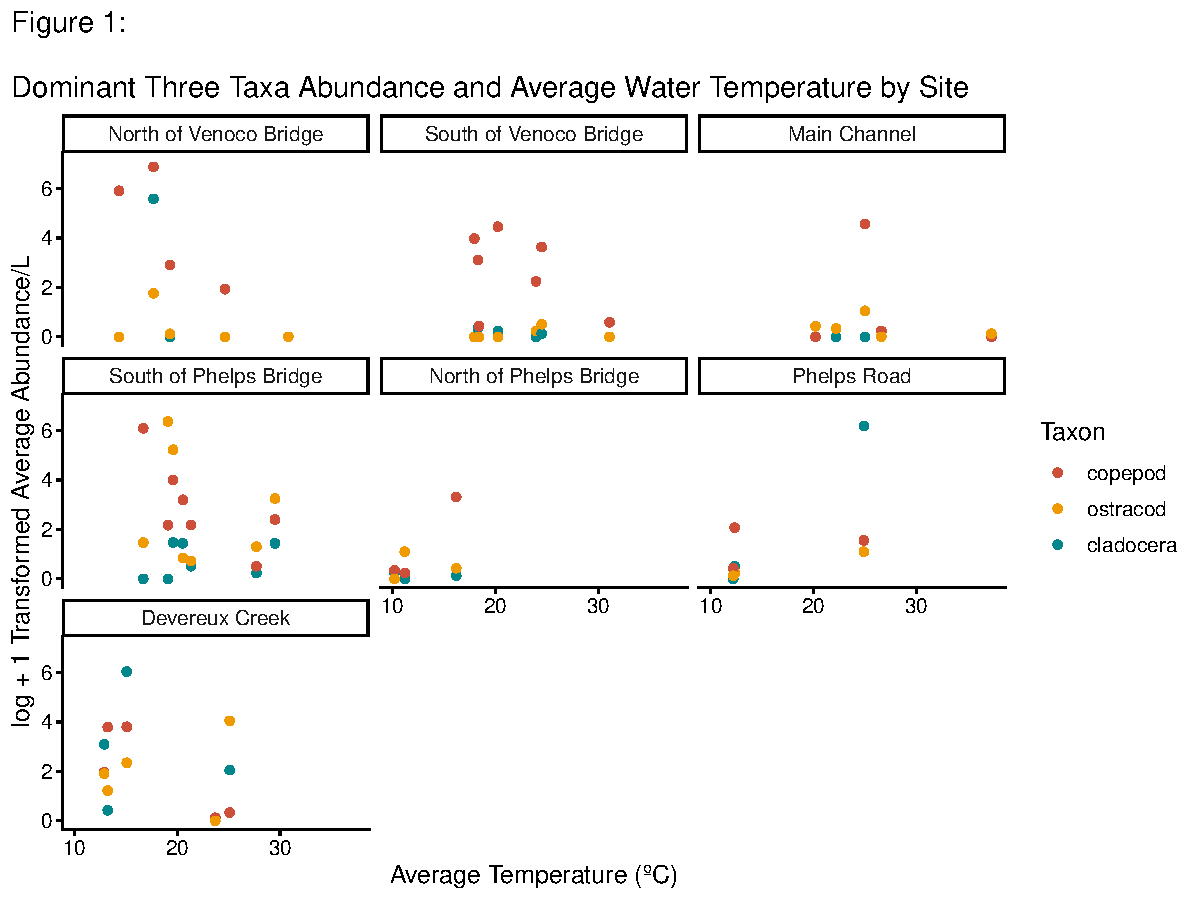
\includegraphics[keepaspectratio]{figure-drafts_files/figure-pdf/scatterplot-1.pdf}}

\subsubsection{Figure 2}\label{figure-2}

\begin{Shaded}
\begin{Highlighting}[]
\NormalTok{figure2 }\OtherTok{\textless{}{-}} \FunctionTok{ggplot}\NormalTok{(}\AttributeTok{data =}\NormalTok{ aq\_ins\_clean,}
                 \FunctionTok{aes}\NormalTok{(}\AttributeTok{x =}\NormalTok{ taxon,}
                     \AttributeTok{y =}\NormalTok{ log\_ave\_lit,}
                     \AttributeTok{color =}\NormalTok{ taxon)) }\SpecialCharTok{+}
  
  \FunctionTok{geom\_jitter}\NormalTok{(}\AttributeTok{height =} \DecValTok{0}\NormalTok{,}
              \AttributeTok{alpha =} \DecValTok{1}\NormalTok{,}
              \AttributeTok{width =} \FloatTok{0.2}\NormalTok{,}
              \AttributeTok{shape =} \DecValTok{21}\NormalTok{) }\SpecialCharTok{+}
  \CommentTok{\# second layer: points to represent medians}
  \FunctionTok{stat\_summary}\NormalTok{(}\AttributeTok{geom =} \StringTok{"point"}\NormalTok{,}
               \AttributeTok{fun =} \StringTok{"mean"}\NormalTok{,}
               \AttributeTok{size =} \DecValTok{4}\NormalTok{,}
               \AttributeTok{color =} \StringTok{"black"}\NormalTok{,}
               \AttributeTok{shape =} \DecValTok{18}\NormalTok{) }\SpecialCharTok{+} \CommentTok{\# 18 = filled diamond }
  
   \FunctionTok{stat\_summary}\NormalTok{(}\AttributeTok{geom =} \StringTok{"errorbar"}\NormalTok{,}
               \AttributeTok{fun.data =}\NormalTok{ mean\_se,}
               \AttributeTok{width =} \FloatTok{0.1}\NormalTok{,}
               \AttributeTok{color =} \StringTok{"black"}\NormalTok{) }\SpecialCharTok{+}
  
  \FunctionTok{scale\_color\_manual}\NormalTok{(}\AttributeTok{values =}\NormalTok{ taxon\_cols) }\SpecialCharTok{+}
  \FunctionTok{labs}\NormalTok{(}\AttributeTok{x =} \StringTok{"Taxon"}\NormalTok{,}
       \AttributeTok{y =} \StringTok{"log + 1 transformed average abundance/L"}\NormalTok{,}
       \AttributeTok{title =} \StringTok{"Figure 2:}

\StringTok{Mean and Distribution of Average Abundance for Three Dominant Taxa"}\NormalTok{)}

\NormalTok{figure2}
\end{Highlighting}
\end{Shaded}

\pandocbounded{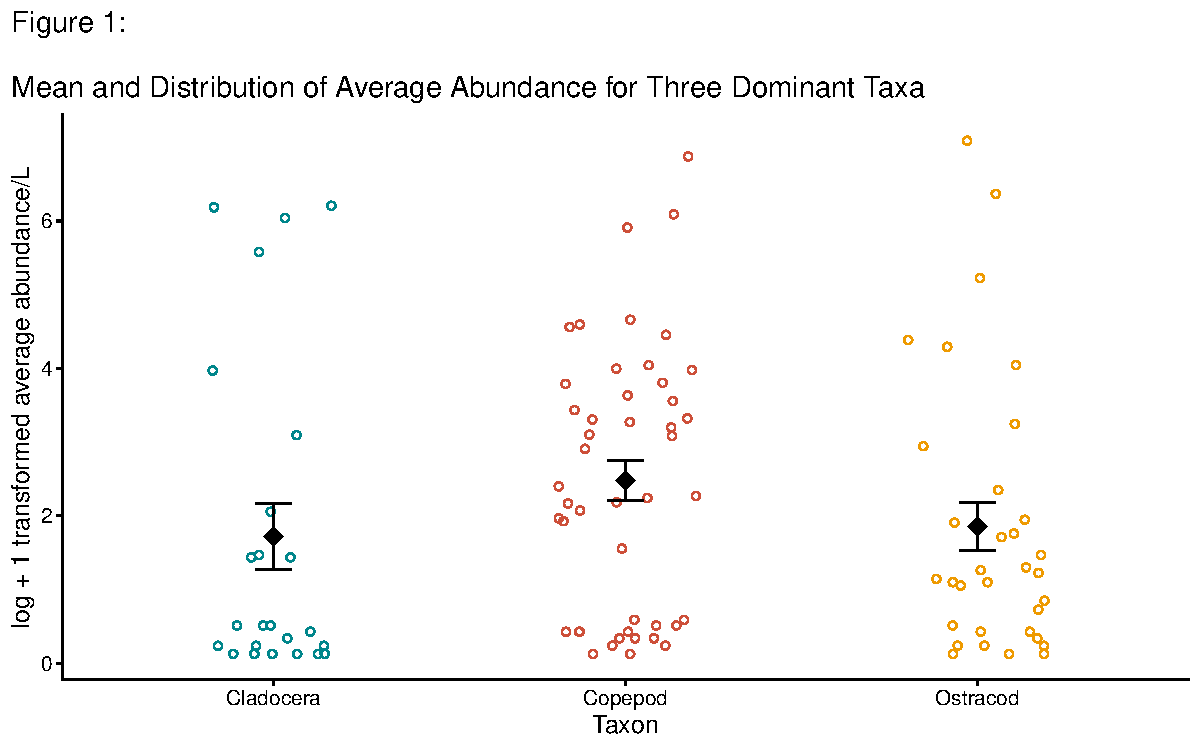
\includegraphics[keepaspectratio]{figure-drafts_files/figure-pdf/strip-chart-1.pdf}}

\subsubsection{Figure 3a}\label{figure-3a}

\begin{Shaded}
\begin{Highlighting}[]
\CommentTok{\# create new object to store figure 4}
\NormalTok{figure3a }\OtherTok{\textless{}{-}} \FunctionTok{ggplot}\NormalTok{(}\AttributeTok{data =}\NormalTok{ aq\_ins\_clean,}
                   \AttributeTok{mapping =} \FunctionTok{aes}\NormalTok{(}\AttributeTok{x =}\NormalTok{ med\_temp,}
                                 \AttributeTok{y =}\NormalTok{ log\_ave\_lit)) }\SpecialCharTok{+}
  
  \FunctionTok{geom\_point}\NormalTok{() }\SpecialCharTok{+} 

  \FunctionTok{facet\_wrap}\NormalTok{(}\SpecialCharTok{\textasciitilde{}}\NormalTok{taxon,}
             \AttributeTok{scales =} \StringTok{"free"}\NormalTok{) }\SpecialCharTok{+}
  
  \FunctionTok{theme}\NormalTok{(}\AttributeTok{legend.position =} \StringTok{"right"}\NormalTok{)}\SpecialCharTok{+}
  
  \FunctionTok{labs}\NormalTok{(}\AttributeTok{title =} \StringTok{"Figure 3a:}

\StringTok{Average Abundance and Average Water Temperature for Three Dominant Taxa"}\NormalTok{,}
       \AttributeTok{x =} \StringTok{"Average Temperature (ºC)"}\NormalTok{,}
       \AttributeTok{y =} \StringTok{"log + 1 Transformed Average Abundance/L"}\NormalTok{,}
       \AttributeTok{color =} \StringTok{"Site"}\NormalTok{)}
  
  
\NormalTok{figure3a}
\end{Highlighting}
\end{Shaded}

\pandocbounded{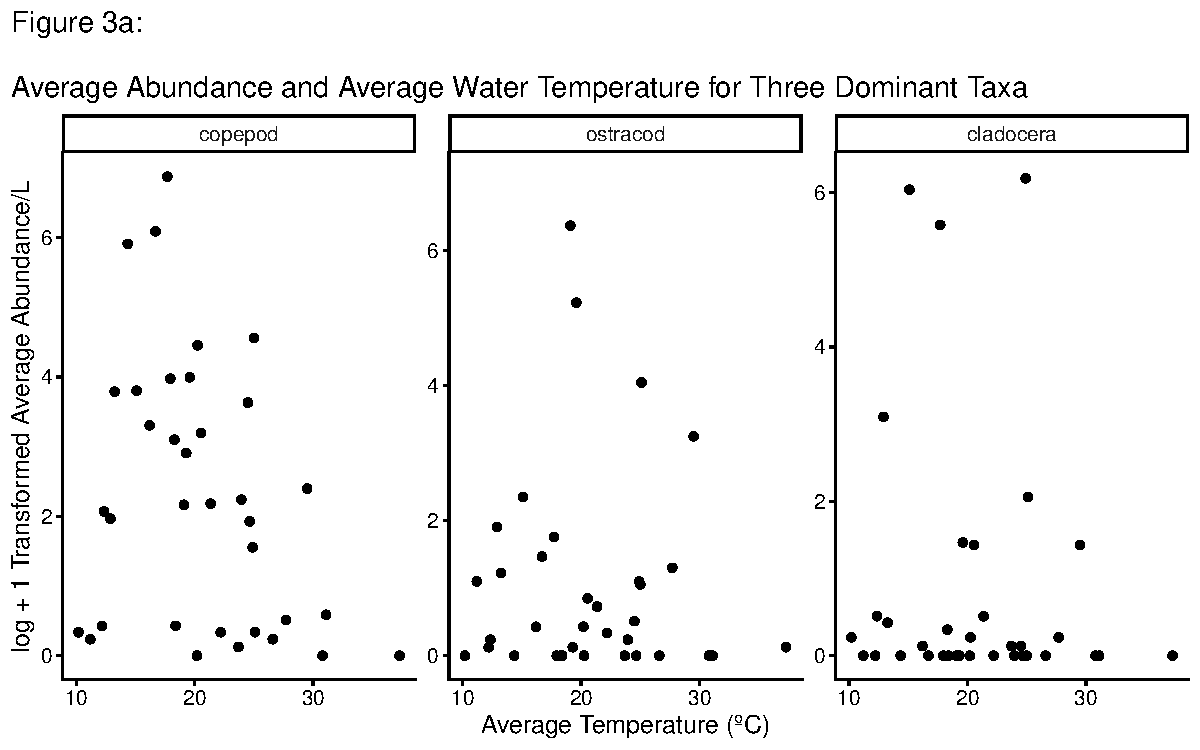
\includegraphics[keepaspectratio]{figure-drafts_files/figure-pdf/figure 3a-1.pdf}}

\subsubsection{Figure 3b}\label{figure-3b}

\begin{Shaded}
\begin{Highlighting}[]
\CommentTok{\# create new object to store figure 3b}
\NormalTok{figure3b }\OtherTok{\textless{}{-}} \FunctionTok{ggplot}\NormalTok{(}\AttributeTok{data =}\NormalTok{ aq\_ins\_clean,}
                   \AttributeTok{mapping =} \FunctionTok{aes}\NormalTok{(}\AttributeTok{x =}\NormalTok{ site,}
                                 \AttributeTok{y =}\NormalTok{ log\_ave\_lit,}
                                 \AttributeTok{color =}\NormalTok{ site)) }\SpecialCharTok{+}
  
  \FunctionTok{geom\_point}\NormalTok{() }\SpecialCharTok{+} 

  \FunctionTok{facet\_wrap}\NormalTok{(}\SpecialCharTok{\textasciitilde{}}\NormalTok{taxon,}
             \AttributeTok{scales =} \StringTok{"free"}\NormalTok{) }\SpecialCharTok{+}
  
  \FunctionTok{theme}\NormalTok{(}\AttributeTok{legend.position =} \StringTok{"right"}\NormalTok{) }\SpecialCharTok{+}
  
  \FunctionTok{scale\_color\_manual}\NormalTok{(}\AttributeTok{values =}\NormalTok{ sites\_cols) }\SpecialCharTok{+}
  
  \FunctionTok{labs}\NormalTok{(}\AttributeTok{title =} \StringTok{"Figure 3b:}

\StringTok{Average Abundance and Average Water Temperature for Three Dominant Taxa}
\StringTok{by Site"}\NormalTok{,}
       \AttributeTok{x =} \StringTok{"Average Temperature (ºC)"}\NormalTok{,}
       \AttributeTok{y =} \StringTok{"log + 1 Transformed Average Abundance/L"}\NormalTok{,}
       \AttributeTok{color =} \StringTok{"Site"}\NormalTok{) }\SpecialCharTok{+}
  
   \CommentTok{\# wrapping x axis labels}
\FunctionTok{scale\_x\_discrete}\NormalTok{(}\AttributeTok{labels =} \FunctionTok{label\_wrap}\NormalTok{(}\AttributeTok{width =} \DecValTok{15}\NormalTok{))}
  
  
\NormalTok{figure3b}
\end{Highlighting}
\end{Shaded}

\pandocbounded{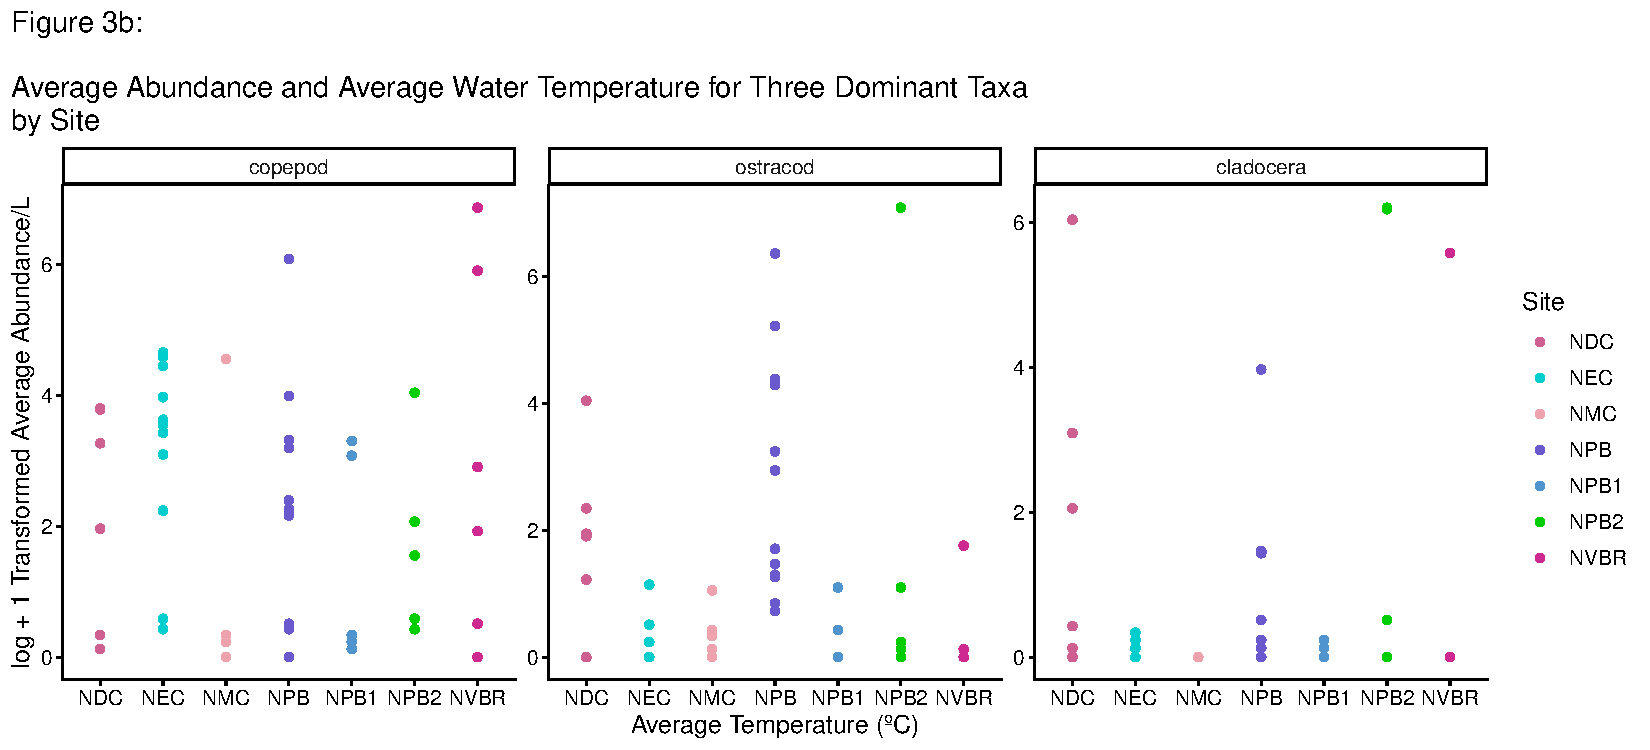
\includegraphics[keepaspectratio]{figure-drafts_files/figure-pdf/figure 3b-1.pdf}}

\subsubsection{Figure 4}\label{figure-4}

\begin{Shaded}
\begin{Highlighting}[]
\CommentTok{\# create new object to store figure 4}
\NormalTok{figure4 }\OtherTok{\textless{}{-}} \FunctionTok{ggplot}\NormalTok{(}\AttributeTok{data =}\NormalTok{ aq\_ins\_clean,}
                   \AttributeTok{mapping =} \FunctionTok{aes}\NormalTok{(}\AttributeTok{x =}\NormalTok{ med\_temp,}
                                 \AttributeTok{y =}\NormalTok{ log\_ave\_lit,}
                                 \AttributeTok{color =}\NormalTok{ taxon)) }\SpecialCharTok{+}
  
  \FunctionTok{geom\_point}\NormalTok{() }\SpecialCharTok{+} 

  \FunctionTok{facet\_wrap}\NormalTok{(}\SpecialCharTok{\textasciitilde{}}\NormalTok{season,}
             \AttributeTok{scales =} \StringTok{"free"}\NormalTok{) }\SpecialCharTok{+}
  \FunctionTok{labs}\NormalTok{(}\AttributeTok{title =} \StringTok{"Figure 4:}

\StringTok{Average Abundance and Average Water Temperature by Season for Three Dominant Taxa"}\NormalTok{,}
       \AttributeTok{x =} \StringTok{"Average Temperature (ºC)"}\NormalTok{,}
       \AttributeTok{y =} \StringTok{"log + 1 Transformed Average Abundance/L"}\NormalTok{,}
       \AttributeTok{color =} \StringTok{"Taxon"}\NormalTok{) }\SpecialCharTok{+}

  \FunctionTok{scale\_color\_manual}\NormalTok{(}\AttributeTok{values =}\NormalTok{ taxon\_cols) }\SpecialCharTok{+}
  
  \FunctionTok{theme}\NormalTok{(}\AttributeTok{legend.position =} \StringTok{"right"}\NormalTok{)}


\NormalTok{figure4}
\end{Highlighting}
\end{Shaded}

\pandocbounded{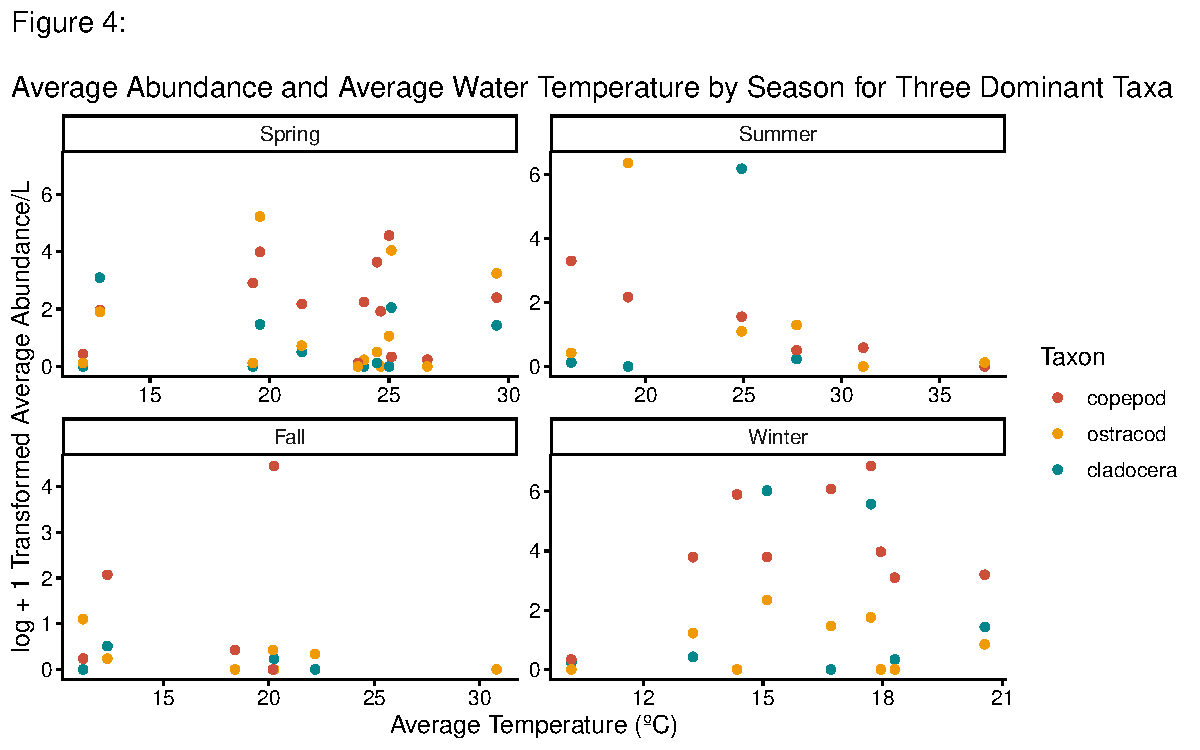
\includegraphics[keepaspectratio]{figure-drafts_files/figure-pdf/season graph-1.pdf}}

\subsection{Other exploratory
visualizations}\label{other-exploratory-visualizations}

\textbf{BELOW PASTE IN THE OTHER EXPLORATORY VISUALS}

\begin{Shaded}
\begin{Highlighting}[]
\CommentTok{\# creating new object for ridgeline}
\NormalTok{ridges }\OtherTok{\textless{}{-}} \FunctionTok{ggplot}\NormalTok{(}\AttributeTok{data =}\NormalTok{ aq\_ins\_clean,}
                 \CommentTok{\# x{-}axis: avg temp}
                 \CommentTok{\# y{-}axis: avg abund}
                 \CommentTok{\# fill geometries by site}
                 \AttributeTok{mapping =} \FunctionTok{aes}\NormalTok{(}\AttributeTok{x =}\NormalTok{ log\_ave\_lit,}
                               \AttributeTok{y =}\NormalTok{ taxon,}
                               \AttributeTok{fill =}\NormalTok{ taxon)) }\SpecialCharTok{+}
  \CommentTok{\# ridges (scale makes ridges shorter so that they don\textquotesingle{}t overlap)}
  \FunctionTok{geom\_density\_ridges}\NormalTok{(}\AttributeTok{scale =} \FloatTok{0.8}\NormalTok{) }\SpecialCharTok{+}
  
  \CommentTok{\# adding means and 95\% confidence intervals}
  \FunctionTok{stat\_summary}\NormalTok{(}\AttributeTok{geom =} \StringTok{"pointrange"}\NormalTok{,}
               \AttributeTok{fun.data =}\NormalTok{ mean\_cl\_normal,}
               \AttributeTok{size =} \FloatTok{0.75}\NormalTok{,}
               \AttributeTok{linewidth =} \DecValTok{1}\NormalTok{) }\SpecialCharTok{+}
  \CommentTok{\# filling geometries with color}
  \FunctionTok{scale\_fill\_manual}\NormalTok{(}\AttributeTok{values =}\NormalTok{ sites\_cols) }\SpecialCharTok{+}
  \CommentTok{\# setting y{-}axis expansions}
  \FunctionTok{scale\_y\_discrete}\NormalTok{(}\AttributeTok{expand =} \FunctionTok{expansion}\NormalTok{(}\AttributeTok{mult =} \FunctionTok{c}\NormalTok{(}\FloatTok{0.01}\NormalTok{, }\FloatTok{0.15}\NormalTok{))) }\SpecialCharTok{+}
  \CommentTok{\# relabelling x{-} and y{-}axis}
  \FunctionTok{labs}\NormalTok{(}\AttributeTok{x =} \StringTok{"avg"}\NormalTok{,}
       \AttributeTok{y =} \StringTok{"taxon"}\NormalTok{)}

\CommentTok{\# displaying object}
\NormalTok{ridges}
\end{Highlighting}
\end{Shaded}

\pandocbounded{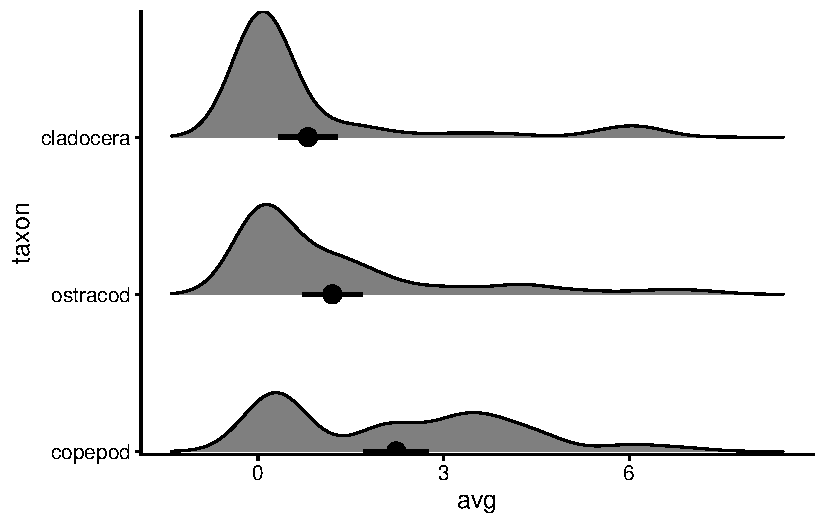
\includegraphics[keepaspectratio]{figure-drafts_files/figure-pdf/exploratory-ridgeline-plot-1.pdf}}

\subsection{Ideas of Analysis for
Background}\label{ideas-of-analysis-for-background}

\begin{itemize}
\tightlist
\item
\end{itemize}

\subsection{Plan for elective}\label{plan-for-elective}

Timeline

Week 7:

\begin{itemize}
\tightlist
\item
  Research all three organisms (copepod, ostracod, cladoceran)
\item
  Gather reference images
\item
  Review your figures
\item
  Take notes on what each figure shows about the species
\item
  Brainstorm collage/drawing style and decide on materials (digital
  vs.~physical).
\end{itemize}

Week 8 * timeline check-in*:

\begin{itemize}
\tightlist
\item
  Have a rough sketch/draft of all three 2D collages-- one per organism
\item
  Bring your notes on what the figures show about each species. This is
  our plan and draft milestone.
\end{itemize}

Week 9:

\begin{itemize}
\tightlist
\item
  Refine and finalize the artwork for 1--2 of the organisms
\item
  Fill in your species notes with complete observations from your
  figures.
\end{itemize}

Week 10:

\begin{itemize}
\tightlist
\item
  Complete the third organism's artwork and finish all species notes
\item
  Do a full review, make sure each collage clearly reflects what your
  figures show about that species.
\end{itemize}

Finals week:

\begin{itemize}
\tightlist
\item
  Final polish, compile everything together
\item
  Present your completed 2D collage triptych with notes.
\end{itemize}

\pandocbounded{
\includegraphics[keepaspectratio]{./Users/lindamarieherrera/github/envs193dd-final-project/code/ostracods-research.png}}




\end{document}
